\documentclass[11pt]{beamer}
\usetheme{Warsaw}
\usepackage[utf8]{inputenc}
\usepackage{amsmath}
\usepackage{amsfonts}
\usepackage{amssymb}
\usepackage{graphicx}
\author{Arnaud Hurel \& Tarik Dadi}
\title[SymCity \hspace{25mm} \insertframenumber/\inserttotalframenumber]{Analyse de papier scientifique : \\SymCity: Feature Selection by Symmetry for Large Scale Image Retrieval}

%\setbeamercovered{transparent} 
\setbeamertemplate{navigation symbols}{}
%\addtobeamertemplate{footline}{\insertframenumber} 
%\logo{} 
%\institute{} 
\date{\today} 
%\subject{} 
\begin{document}

\begin{frame}
\titlepage
\end{frame}

\begin{frame}{Introduction}

This paper presents technics allowing to retrieve all the similar pictures in a dataset of unique views of buildings or urban scenes by extracting the most accurate features.\newline

Current problems:
\begin{itemize}
\item feature selection
\item vocabulary learning
\item location and landmark recognition
\item structure from motion and 3D reconstruction
\item learning process relying on wide baseline matching on multiple views of the same object
\end{itemize}

Useful technics to select features within a single image:
\begin{itemize}
\item self-similaries
\item symmetries
\item repeating patterns
\end{itemize}
\end{frame}

\begin{frame}
\tableofcontents
\end{frame}

\begin{frame}
\frametitle{Paper presentation}
\section{Paper presentation}

\subsection{Bag of Words (BoW)}
Bag of Words (features + descriptors) + geometry verification :
\begin{itemize}
\item Very successful at particular object retrieval (precise and fast enough)
\item Not for large scale problem
\item Huge memory footprint of the index
\end{itemize}
\vspace{0.3cm}
\subsection{Fisher Kernels}
Fisher Kernels
\begin{itemize}
\item more global representation than BoW
\item not compatible with geometry verification
\item less precise
\end{itemize}

\end{frame}

\begin{frame}
\frametitle{Paper presentation : Feature Selection}
\begin{itemize}
\item Only practical alternative
\item Popular idea : select features from multiple views with a baseline retrieval system
\item Image unique : feature selection by self-similarity
\end{itemize}

$\Rightarrow$ Developpment of two self-matching algorithms based on state of the art spatial matching methods:
\begin{itemize}
\item Fast Spatial Matching (FSM), Philbin \& al.
\item Hough Pyramid Matching (HPM), Tolias \& Avrithis
\end{itemize}

\end{frame}

\begin{frame}
\frametitle{Paper presentation : Feature Selection}
\begin{itemize}
\item Apply the algorithm between each image and either itself or its reflection.
\item Detect \textbf{repeating patterns} or \textbf{local symmetries}
\item Index only the participating features
\item Features repeating within a single image are quite likely to repeat accross different views
\end{itemize}

$\Rightarrow$ This methods are successful with urban image collection.
\end{frame}

\begin{frame}
\begin{center}
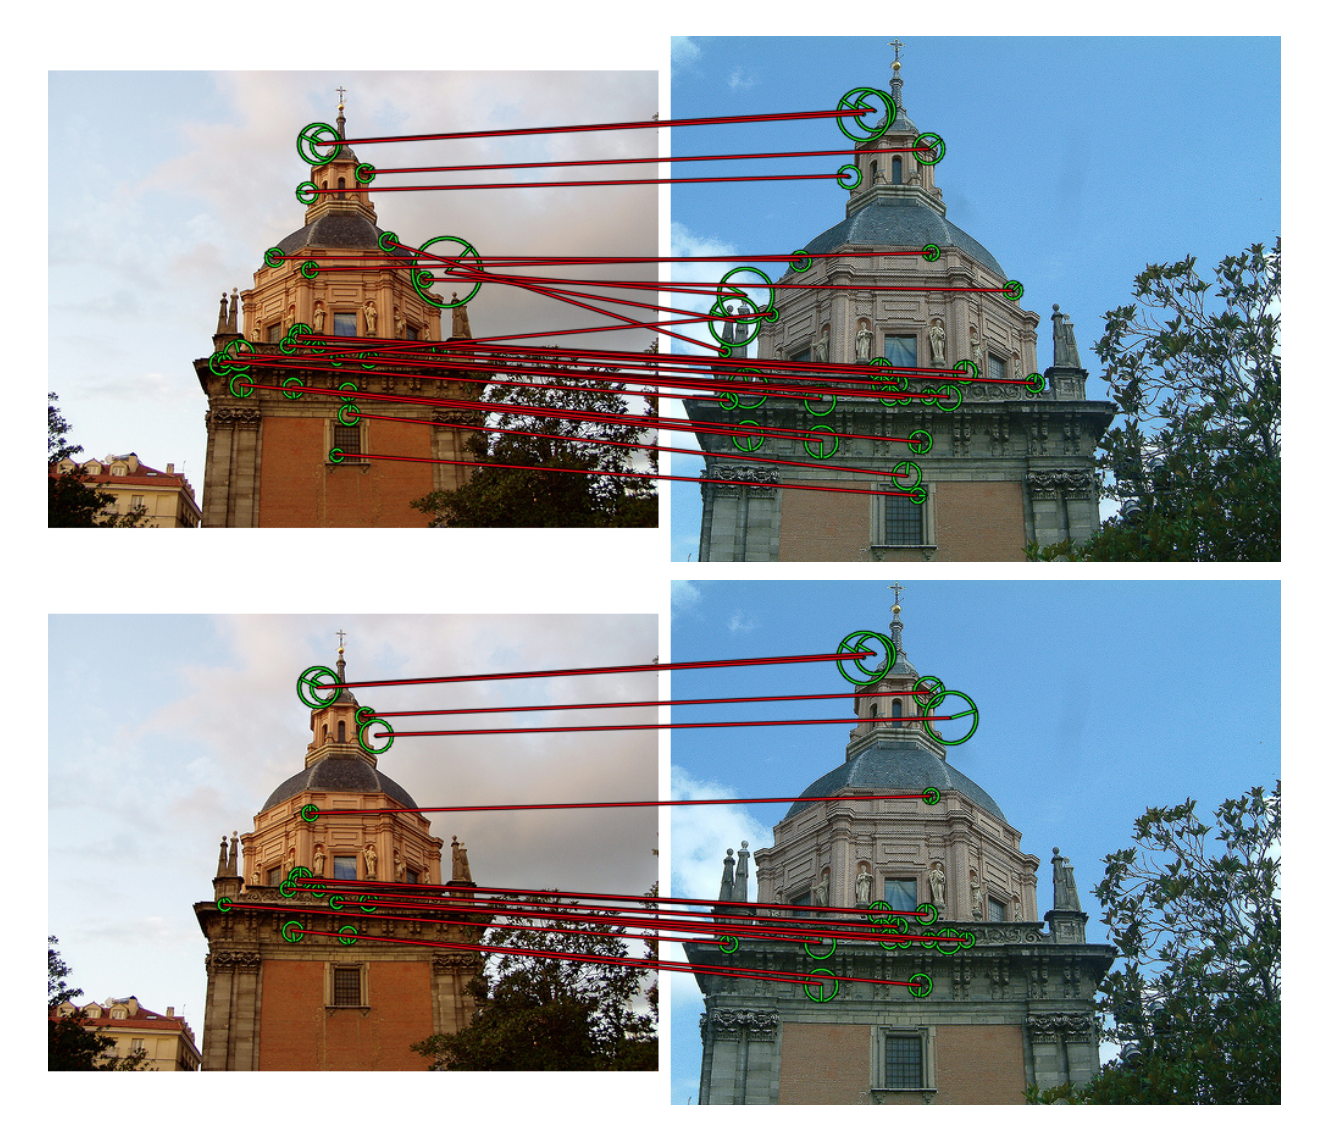
\includegraphics[scale=0.3]{figure1.png}
\end{center}
Left image is considered a query image. Top using all feature, bottom using selected features.
\end{frame}

\begin{frame}
\frametitle{Related Work: Multiple Views}
$\blacktriangleright$ Feature selection has recently become a popular way of reducing index space for image retrieval

\vspace{0.3cm}

Supervised:
\begin{itemize}
\item Schindler \& al. : location recognition
\item Knopp \& al. : local confusion score
\end{itemize}
\vspace{0.3cm}
Unsupervised:
\begin{itemize}
\item Turcot \& Lowe : unsupervised selection of features using spatial verification
\item Naikal \& al. : sparse PCA on covariance matrix of the BoW histogram
\end{itemize}

$\Rightarrow$ Require multiple views of the same object

\end{frame}

\begin{frame}
\frametitle{Related Work: Unique views}
Turcot \& Lowe (first approach of this kind)
\begin{itemize}
\item keep the largest scale features in the index $\Leftrightarrow$ reducing image resolution
\item detect self-similarities, repeating patterns and symmetries to select features
\item approach fails with large scale distractor dataset 
\end{itemize}
\vspace{0.3cm}
Tuytelaars \& al.
\begin{itemize}
\item solution of high complexity
\item find invariant neighborhoods and apply cascaded Hough transform
\item detect collinear intersections
\end{itemize}
\end{frame}
\begin{frame}
\frametitle{Related Work: Unique views}
Cornelius \& al.
\begin{itemize}
\item use of Hough voting
\item do not require image descriptors
\item detect local affine frames (LAFs) from image \& reflection
\item match them using their local geometry
\item allow each matching LAF pair to vote for a symmetry axis
\end{itemize}
\end{frame}

\begin{frame}
\frametitle{Contribution to Feature Selection}
$\blacktriangleright$ 2 alternatives unsupervised methods for feature selection

\vspace{0.3cm}

$\blacktriangleright$ Focusing on geometrically consistent feature groups within a single image, roughly representing reapeating patterns or local symmetries

\vspace{0.3cm}

$\blacktriangleright$ Handling direct and opposite transformation matching
\begin{itemize}
\item direct matching
\item flipped matching
\end{itemize}
\end{frame}

\begin{frame}
\frametitle{Contribution to Feature Selection}
$\blacktriangleright$ symmetry or repeating pattern detection in a single image \newline{} $\Leftrightarrow$ spatial matching between two images

\vspace{0.3cm}
Two issues:
\begin{itemize}
\item Spatial matching usually assumes 1-to-1 correspondance betweet features of two images
\item Seeking robustness against outliers
\end{itemize}
\end{frame}

\begin{frame}
\frametitle{Contribution to Feature Selection : Representation}

$\blacktriangleright$ An image is represented by a set of local features $X$.

\begin{itemize}
\item local feature $x \in X$ 
\item x associated:
\begin{itemize}
\item descriptor $d(x) \in \mathbb{R}^D$
\item position $p(x) \in \mathbb{R}^2$
\item log-scale $\sigma(x) \in \mathbb{R}$
\item orientation $\theta(p) \in [-\pi, \pi]$ 
\end{itemize}
\item represented by a vector
\end{itemize}
\begin{center}
$g(x) = [p(x)^T \sigma(x) \theta(x)]^T$
\end{center}
\end{frame}

\begin{frame}
\frametitle{Contribution to Feature Selection : Representation}
$\blacktriangleright$ The set of tentatives correspondences of X contains pairs of similar features that are also valid:
\begin{center}
$C_t(X) = C_d(X) \bigcap C_v(X) $
\end{center}

With:
\begin{itemize}
\item $C_d(X)$ : set of appearence or descriptor based correspondences of image X
\item $C_v(X)$ : set of valid correspondences 
\end{itemize}
\end{frame}

\begin{frame}
\frametitle{Contribution to Feature Selection : Spatial self-Matching}

lolo


\end{frame}




\begin{frame}
\frametitle{Validation}
Testing the behavior of SSM and HPSM under different parameter settings and compare performance to other feature selection methods for single image.

\vspace{0.3cm}
Used datasets:
\begin{itemize}
\item SymCity: annotated dataset from flickr (953 images)
\item WordCity; distractor dataset (1M images of cities)
\end{itemize}

\end{frame}

\begin{frame}
\frametitle{Validation : Protocol}
$\blacktriangleright$ The experimentation follows this steps:
\begin{enumerate}
\item Extract features and descriptors with SURF algorithm
\item Assign visual word form a generic 100K vocabulary using FLANN
\item Keep only the nearest neighbor under Euclidean disctance
\item Adding more features in case of symmetrie detection failure 
\end{enumerate}
\end{frame}

\begin{frame}
\frametitle{Validation : Key Performance Indicators}
$\blacktriangleright$ Measure retrieval performance by mean Average Precision (mAP) over all queries.

\vspace{0.3cm}
If 1 query = 1 image $\Rightarrow$ $mAP = 1/i$ where $i$ is the rank of the result in the list of image

\vspace{0.3cm}
$\blacktriangleright$ Measure index size by the number of entries in the inverted index per image.

\vspace{0.3cm}
$\blacktriangleright$ Running time refers to the entire process of feature selection for one image including both direct and flipped matching for each method.
\end{frame}

\begin{frame}
\frametitle{Validation : Tuning}

Fixed variables :
\begin{itemize}
\item similarity threshold : $\delta = 0.1$
\item inlier threshold : $\epsilon = 7 pixels$
\item hierarchical level : $L = 5 levels$
\end{itemize}

Tunnable variable :
\begin{itemize}
\item selection threshold for SSM : $\tau_\alpha$
\item selection threshold for HPSM : $\tau_\beta$
\item number $k$ of nearest neigbors
\end{itemize}

\end{frame}

\begin{frame}
\frametitle{Validation : Tuning}
\begin{center}
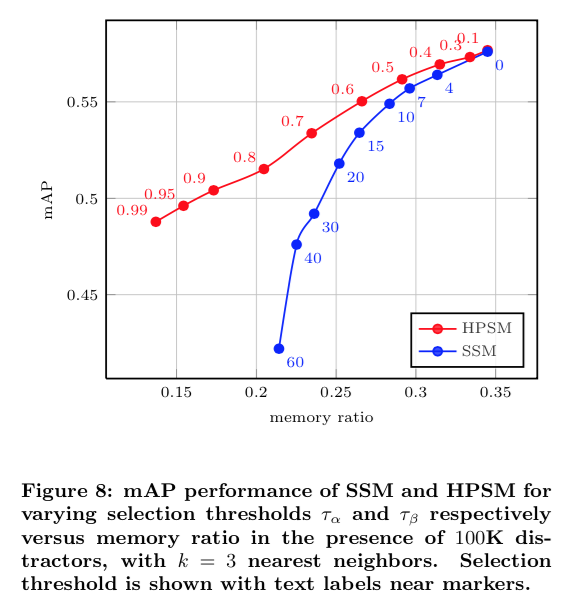
\includegraphics[scale=0.48]{figure8}
\hspace{0.4cm}
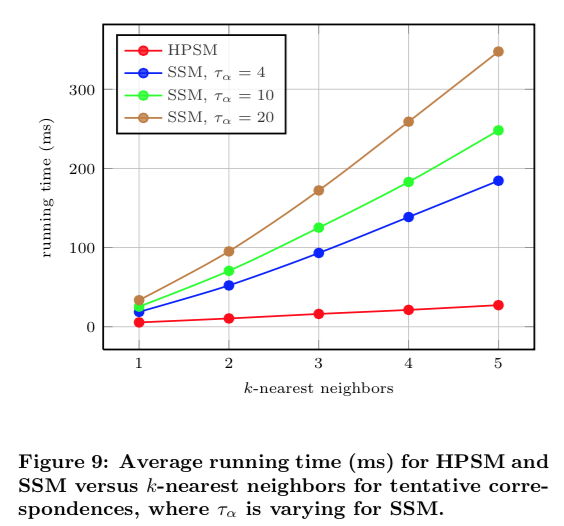
\includegraphics[scale=0.55]{figure9}
\end{center}
\end{frame}

\begin{frame}
\frametitle{Validation : Tuning}
$\blacktriangleright$ HPSM Performance
\begin{center}
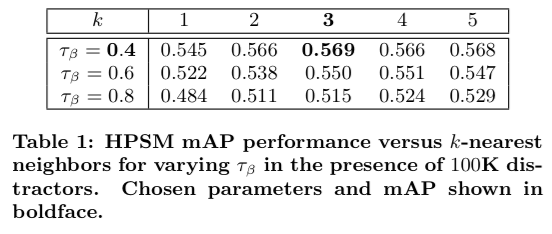
\includegraphics[scale=0.8]{table1}
\end{center}
Best result obtained for $k = 3$ and $\tau_\beta = 0.4$ for an average running time of 16.2 ms
\end{frame}

\begin{frame}
\frametitle{Validation : Comparisons}
\begin{center}
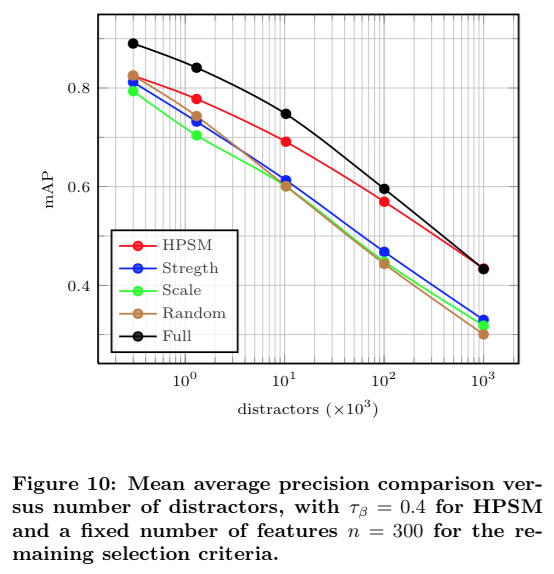
\includegraphics[scale=0.55]{figure10}
\end{center}

\end{frame}

\end{document}